\section{Untimed semantics}
\label{section untimed semantics}
In this section, we present an untimed semantics for MMTs and prove that is equivalent with the timed semantics.
In order to define the untimed semantics, we need to define a number of abstractions of timed runs.

\subsection{Timed and untimed runs and behaviors}
Configurations consists of pairs of states and timer valuations. This means that there are two natural abstractions of
timed runs: an abstraction $\untime$ that forgets all timing information and keeps the transitions of the MMT, 
and an abstraction $\beh$ that forgets information on states and preserves the timing information.
When we compose these abstractions we obtain \emph{untimed behaviors} in which only information about inputs, outputs,
updates and active timers is preserved.
The abstractions commute, $\beh(\untime(\alpha))=\untime(\beh(\alpha))$, and play a key role in
the technical development of this paper.
%
Formally, an \emph{untimed behavior} over inputs $I$ and outputs $O$ is a sequence 
\begin{eqnarray*}
\beta & = & X_0 \xrightarrow{i_1/o_1, \rho_1} X_1  \cdots \xrightarrow{i_k/o_k, \rho_k} X_{k},
\end{eqnarray*}
where $X_0 \subseteq X$ and, for each $j>0$,  $i_j \in \extinputs$, $o_j \in O$, $\rho_j \in X \hookrightarrow \natplus$, and
 $X_j \setminus X_{j-1}  \subseteq \domof{\rho_j} \subseteq X_j \subseteq X$.
Moreover, if $i_j = \toevent{x}$, for some $j>0$, then $x \in X_{j-1}$ and $x \not\in X_j \setminus \domof{\rho_j}$.
%
An \emph{untimed run} of an MMT $\M$ is a sequence
\begin{eqnarray*}
\gamma & = & q_0 \xrightarrow{i_1/o_1, \rho_1} q_1   \cdots \xrightarrow{i_k/o_k, \rho_k} q_k
\end{eqnarray*}
of transitions of $\M$ that starts with the initial state $q_0$. 
To each untimed run $\gamma$ we associate an untimed behavior by replacing all
states by their sets of timers:
\begin{eqnarray*}
\beh(\gamma) & = & \vars(q_0) \xrightarrow{i_1/o_1, \rho_1} \vars(q_1)  \cdots \xrightarrow{i_k/o_k, \rho_k} \vars(q_k).
\end{eqnarray*}
We say that $\beta$ is an untimed behavior of $\M$ if $\M$ has an untimed run $\gamma$ with $\beh(\gamma) = \beta$.
Note that the initial timer set of an untimed behavior of $\M$ is empty.
%
A \emph{timed behavior} over inputs $I$ and outputs $O$ is an alternating sequence
\begin{eqnarray}
\label{timedbehavior}
\sigma & = & \tvals_0 \xrightarrow{d_1} \tvals'_0 \xrightarrow{i_1/o_1, \rho_1} \tvals_1 \cdots
\xrightarrow{d_k} \tvals'_{k-1} \xrightarrow{i_k/o_k, \rho_k} \tvals_{k}
\end{eqnarray}
of delay transitions and discrete transitions with, for each $j$,
$\tvals_j, \tvals'_j$ valuations and,
for each $j>0$,  $d_j \in \delays$, $i_j \in \extinputs$, $o_j \in O$, and $\rho_j \in X \hookrightarrow \natplus$.
To each timed behavior $\sigma$ we associate an untimed behavior by forgetting the
delay transitions and by replacing valuations by their domain:
\begin{eqnarray*}
\untime(\sigma) & = & \domof{\tvals_0} \xrightarrow{i_1/o_1, \rho_1}  \cdots \xrightarrow{i_k/o_k, \rho_k} \domof{\tvals_k}.
\end{eqnarray*}
We say that untimed behavior $\beta$ is \emph{feasible} if there exists a timed behavior $\sigma$ such that $\untime(\sigma) = \beta$.
The following technical lemma follows directly from the definitions:

\begin{lemma}
\label{feasible plus input is feasible}
Suppose $\beta$ is a feasible untimed behavior that ends with timer set $Y$, and 
$Y \xrightarrow{i/o, \rho} Y'$ is an untimed behavior with $i \in I$.
Then $\beta \xrightarrow{i/o, \rho} Y'$ is a feasible untimed behavior.
\end{lemma}

We also associate a timed word to timed behavior $\sigma$ by forgetting valuations, timers, and update functions:
\begin{eqnarray*}
\timedword(\sigma) & = & d_ 1 ~ i'_1 ~ o_1 ~ i'_2 ~ o_2 \cdots d_k ~ i'_k ~ o_k, 
\end{eqnarray*} 
where for all  $j$,
\begin{eqnarray*}
i'_j  & = &  \left\{ \begin{array}{ll}
i_j & \mbox{if } i_j \in I,\\
\mathit{to} & \mbox{if } i_j \in \toevents.
\end{array} \right.
\end{eqnarray*}
Let $\alpha$ be a timed run of an MMT $\M$: 
\begin{eqnarray*}
\alpha & = & (q_0, \tvals_0) \xrightarrow{d_1} (q_0, \tvals'_0) \xrightarrow{i_1/o_1} (q_1, \tvals_1)  \cdots
 \xrightarrow{i_k/o_k} (q_k, \tvals_k).
\end{eqnarray*}
Then $\alpha$ can be projected both to an untimed run of $\M$
\begin{eqnarray*}
\untime (\alpha) & = & q_0 \xrightarrow{i_1/o_1, \rho_1} q_1  \cdots \xrightarrow{i_k/o_k, \rho_k} q_k
\end{eqnarray*}
(the $\rho_j$'s are determined since $\M$ is deterministic) and to a timed behavior
\begin{eqnarray*}
\beh(\alpha) & = & \tvals_0 \xrightarrow{d_1} \tvals'_0 \xrightarrow{i_1/o_1, \rho_1} \tvals_1  \cdots
\xrightarrow{d_k} \tvals'_{k-1} \xrightarrow{i_k/o_k, \rho_k} \tvals_{k}.
\end{eqnarray*}
\iflong
We say that $\sigma$ is an timed behavior of $\M$ if $\M$ has an timed run $\alpha$ with $\beh(\alpha) = \sigma$.
\fi
Note that $\beh(\untime(\alpha))=\untime(\beh(\alpha))$ and $\timedword(\alpha) = \timedword(\beh(\alpha))$.
\iflong
Thus the diagram of Figure~\ref{fig:diagram}, which summarizes the various types of runs and behaviors that we consider
in this article, commutes.
\begin{figure}[h]
\centering
\begin{tikzpicture}[->,>=stealth',shorten >=1pt,auto,node distance=2.5cm,main node/.style={circle,draw,font=\sffamily\large\bfseries}]
  \node[state,align=center] (1) {timed \\ runs of\\ $\M$};
  \node[state,align=center] (2) [below of=1] {untimed \\ runs of\\ $\M$};
  \node[state,align=center] (3) [right of=1] {timed\\ behaviors};
  \node[state,align=center] (4) [right of=2] {untimed\\ behaviors};
  \node[state,align=center] (5) [right of=3] {timed \\words};

  \path[every node/.style={font=\sffamily\scriptsize}]
    (1) edge  node {$\untime$} (2)
        edge  node {$\beh$} (3)
        edge[bend left=40]  node {$\timedword$} (5)
    (2) edge  node {$\beh$} (4)
    (3) edge  node {$\untime$} (4)
        edge  node {$\timedword$} (5);
\end{tikzpicture}
\caption{Relating different types of runs and behaviors}
\label{fig:diagram}
\end{figure}
\fi
Conversely, if $\gamma$ is an untimed run  of $\M$ and $\sigma$ is a timed behavior such that $\beh(\gamma) = \untime(\sigma)$,
then there exists a unique timed run $\alpha$ of $\M$ with $\untime(\alpha) = \gamma$ and $\beh(\alpha) = \sigma$.
We refer to $\alpha$ as $\run(\gamma,\sigma)$.

For any nonempty sequence $\sigma$, $\Head{\sigma}$ denotes the first element, $\Tail{\sigma}$ denotes the sequence obtained by removing the first element, and $\Last{\sigma}$ denotes the last element.
Suppose $\beta, \beta'$ are untimed behaviors over $I$ and $O$ such that $\Last{\beta} = \Head{\beta'}$.
Then the \emph{sequential composition} of $\beta$ and $\beta'$, written $\beta \cdot \beta'$, is the untimed behavior $\beta ~ \Tail{\beta'}$.
Behavior $\beta$ is a \emph{prefix} of behavior $\gamma$ if there exists an behavior $\beta'$ such that $\gamma = \beta \cdot \beta'$.

\subsection{Definition untimed semantics}
We would, intuitively, like to define the untimed semantics of an MMT $\M$ as the set of its feasible untimed behaviors.
However, this semantics would then depend heavily on the identity of the timers. Therefore, we define an equivalence relation
on untimed behaviors, which deems two untimed behaviors equivalent if there is a consistent renaming of timers that transforms
the one into the other.

Let $\beta$ and $\beta'$ be two untimed behaviors with the same length and outputs:
\begin{eqnarray*}
\beta & = & X_0 \xrightarrow{i_1/o_1, \rho_1} X_1  \xrightarrow{i_2/o_2, \rho_2} X_2 \cdots \xrightarrow{i_k/o_k, \rho_k} X_{k},\\
\beta' & = & Y_0 \xrightarrow{i'_1/o_1, \rho'_1} Y_1  \xrightarrow{i'_2/o_2, \rho'_2} Y_2 \cdots \xrightarrow{i'_k/o_k, \rho'_k} Y_{k}.
\end{eqnarray*}
An \emph{isomorphism} from $\beta$ to $\beta'$ is a list $f = f_0 ,\ldots, f_k$ of bijections $f_j : X_j \rightarrow Y_j$ such that
for all $j>0$: (1) for all $x \in X_j \setminus \domof{\rho_j})$, $f_j(x)=f_{j-1}(x)$,
(2) $i'_j = i_j$ if $i_j \in I$ and $i'_j = \toevent{f_{j-1}(x)}$ if $i_j = \toevent{x}$, for some $x \in X_{j-1}$, and
(3) $\domof{\rho'_j} = f_j(\domof{\rho_j})$ and $\rho'_j(y) = \rho_j ( f_j^{-1}(y))$, for all $y\in\domof{\rho'_j}$.
In this case, since $\beta'$ is fully determined by $\beta$ and $f$, we write $\beta' = f(\beta)$.
We say that $\beta$ and $\beta'$ are \emph{isomorphic} if there exists an isomorphism $f$ from $\beta$ to $\beta'$.
Two sets of untimed behaviors $A$ and $B$ are \emph{isomorphic} if for each untimed behavior of $A$ there is an isomorphic untimed behavior in $B$,
and vice versa.

Isomorphisms can be lifted to timed behaviors in the obvious way. 
Let $\sigma$ and $\sigma'$ be two timed behaviors with the same length and outputs:
\begin{eqnarray*}
\sigma & = & \tvals_0 \xrightarrow{d_1} \tvals'_0 \xrightarrow{i_1/o_1, \rho_1} \tvals_1  \cdots
\xrightarrow{d_k} \tvals'_{k-1} \xrightarrow{i_k/o_k, \rho_k} \tvals_{k},\\
\sigma' & = & \lambda_0 \xrightarrow{d_1} \lambda'_0 \xrightarrow{i'_1/o_1, \rho'_1} \lambda_1  \cdots
\xrightarrow{d_k} \lambda'_{k-1} \xrightarrow{i'_k/o_k, \rho'_k} \lambda_{k}.
\end{eqnarray*}
An \emph{isomorphism} from $\sigma$ to $\sigma'$ is a list $f = f_0 ,\ldots, f_k$ of bijections such that
(1) $f$ is an isomorphism from $\untime(\sigma)$ to $\untime(\sigma')$, and
$\lambda_j = \kappa_j \circ f_j^{-1}$ and $\lambda'_j = \kappa'_j \circ f_j^{-1}$, for all $j$.
Since $\sigma'$ is fully determined by $\sigma$ and $f$, we write $\sigma' = f(\sigma)$.
Two timed behaviors $\sigma$ and $\sigma'$ are \emph{isomorphic} if there exists an isomorphism $f$ from $\sigma$ to $\sigma'$.
Since an isomorphism only renames timers, which do not appear in timed words, 
isomorphic timed behaviors induce identical timed words: $\sigma' = f(\sigma) \Rightarrow \timedword(\sigma') = \timedword(\sigma)$.

The following lemmas follow directly from the definitions:
\begin{lemma}
\label{lemma isomorphism}
Let $\sigma$ be a timed behavior and let $f$ be an isomorphism for $\sigma$.
Then $\untime(f(\sigma)) = f(\untime(\sigma))$.
\end{lemma}
\begin{lemma}
If untimed behaviors $\beta$ and $\beta'$ are isomorphic, then $\beta$ is feasible iff $\beta'$ is feasible.
\end{lemma}

Two MMTs $\M$ and $\N$ with the same sets of inputs are \emph{untimed equivalent}, denoted $\M \approx_{\mathit{untimed}} \N$, iff their sets of feasible untimed behaviors are isomorphic. The following basic property will be needed later on:

\begin{lemma}
\label{not untimed}
Suppose $\M, \N$ are MMTs with $\M \not\approx_{\mathit{untimed}} \N$.
Then there exists a feasible untimed behavior $\beta$ of $\M$ that is not isomorphic to any feasible untimed behavior of $\N$.
\end{lemma}

Untimed equivalence is finer than timed equivalence:

\begin{theorem}
\label{untimedimpliestimed}
$\M \approx_{\mathit{untimed}} \N$
implies
$\M \approx_{\mathit{timed}} \N$.
\end{theorem}
\iflong
\begin{proof}
Assume $\M \approx_{\mathit{untimed}} \N$ and $w$ is a timed word of $\M$.
Since $\approx_{\mathit{timed}}$ is symmetric, it suffices to prove that $w$ is a timed word of $\N$.
Since $w$ is a timed word of $\M$,
there exists a timed run $\alpha$ of $\M$ with $\timedword(\alpha) = w$. 
Let $\sigma = \beh(\alpha)$ and $\beta = \untime(\sigma)$. 
Then $\beta$ is a feasible untimed behavior of $\M$ and $\timedword(\sigma) = w$.
Since  $\M \approx_{\mathit{untimed}} \N$, there exists an isomorphism $f$ such that 
$\beta' = f(\beta)$ is a feasible untimed behavior of $\N$.
Hence $\N$ has an untimed run $\gamma'$ such that $\untime(\gamma') = \beta'$.
Let $\sigma' = f(\sigma)$.
By Lemma~\ref{lemma isomorphism}, $\sigma'$ is a timed behavior with 
$\untime(\sigma') = \untime(f(\sigma)) = f(\untime(\sigma)) = f(\beta) = \beta'$.
Since $\beh(\gamma') = \untime(\sigma') = \beta'$, $\N$ has a timed run $\alpha' = \run(\gamma',\sigma')$ with
$\beh(\alpha') = \sigma'$.
Note that $\timedword(\alpha') = \timedword(\sigma') = \timedword(f(\sigma)) = \timedword(\sigma) = w$.
Hence $w$ is a timed word of $\N$, as required.
\end{proof}
\fi
The converse of Theorem~\ref{untimedimpliestimed} does not hold. 
%The two MMTs of Figure~\ref{fig:twoequivalentone}, for instance,
%are timed equivalent but not untimed equivalent,
%because the top MMT has an untimed behavior
%$ \emptyset \xrightarrow{i/o,~ x, y:=1,2 } \{ x, y \}$, for which the bottom MMT has no isomorphic behavior.
%\begin{figure}
%\ifshort
%\vspace{-1em}
%\fi
%\begin{center}
%\begin{tikzpicture}[->,>=stealth',shorten >=1pt,auto,node distance=3cm,main node/.style={circle,draw,font=\sffamily\large\bfseries}]
%  \node[initial, state] (1) {$q_0$};
%  \node[state] (2) [right of=1] {$q_1$};
%  \node[state] (3) [right of=2] {$q_2$};
%  \node[state] (4) [right of=3] {$q_3$};
%
%  \path[every node/.style={font=\sffamily\scriptsize}]
%    (1) edge node {$i/o$, $x, y:=1,2$} (2)  
%    (2) edge  node {$\toevent{x}/o'$} (3)
%   (3) edge node {$\toevent{y}/o''$} (4);
%\end{tikzpicture}
%
%\begin{tikzpicture}[->,>=stealth',shorten >=1pt,auto,node distance=3cm,main node/.style={circle,draw,font=\sffamily\large\bfseries}]
%  \node[initial, state] (1) {$q_0$};
%  \node[state] (2) [right of=1] {$q_1$};
%  \node[state] (3) [right of=2] {$q_2$};
%  \node[state] (4) [right of=3] {$q_3$};
%
%  \path[every node/.style={font=\sffamily\scriptsize}]
%    (1) edge node {$i/o$, $x:=1$} (2)  
%    (2) edge  node {$\toevent{x}/o'$, $x:=1$} (3)
%   (3) edge node {$\toevent{x}/o''$} (4);
%\end{tikzpicture}
%\caption{Timed equivalent but not untimed equivalent}
%\label{fig:twoequivalentone}
%\end{center}
%\end{figure}
%For this reason, we restrict ourselves in the rest of this article to MMTs in which at most
%one clock can be (re)set in a single transition. This restriction has the additional advantage that it
%eliminates the uncontrollable nondeterminism illustrated in Figure~\ref{fig:nondeterminism}.
% and \ref{fig:nondeterminism2}.
%Provided there is no uncontrollable nondeterminism, most MMTs
%have an equivalent MMT that (re)sets at most one timer per transition:
%if multiple timers are started simultaneously then we can often encode this by just
%starting the timer $x$ with the smallest value $d_0$, and recording the set of remaining timers in the discrete state.
%Then, when $x$ expires, we start the next timer (with timeout value decremented by $d_0$), etc.
%However, such an encoding is not always possible. 
%\iflong
%Figure~\ref{fig:counterexample} presents an example of an MMT for which no equivalent MMT exists
%in which at most one timer is (re)set per transition.
%\begin{figure}
%\begin{center}
%\begin{tikzpicture}[->,>=stealth',shorten >=1pt,auto,node distance=2.7cm,main node/.style={circle,draw,font=\sffamily\large\bfseries}]
%  \node[initial, state] (1) {$q_0$};
%  \node[state] (2) [right of=1] {$q_1$};
%  \node[state] (3) [right of=2] {$q_2$};
%  \node[state] (4) [below of=3] {$q_3$};
%  \node[state] (5) [below of=2] {$q_4$};
%
%  \path[every node/.style={font=\sffamily\scriptsize}]
%    (1) edge node {$i/o$, $x, y:=1,2$} (2)  
%    (2) edge  node {$i/o$} (3)
%   (3) edge node {$\toevent{y}/o''$} (4)
%   (2) edge node {$\toevent{x}/o'$} (5);
%\end{tikzpicture}
%\caption{Starting more than one timer on a transition increases expressivity}
%\label{fig:counterexample}
%\end{center}
%\end{figure}
%\fi
%
%Even when we restrict to MMTs that may (re)set at most one timer per transition, there is a difference
%between the timed and the untimed semantics.
This is due to the fact that an MMT may have timers that are always stopped or restarted before
they expire. Such ``ghost'' timers are visible in the untimed semantics but cannot be observed in the timed semantics.
\iflong
Figure~\ref{fig:ghosttimers} gives an example of an MMT with a ghost timer. The MMT is equivalent to the MMT obtained by 
omitting the update $y :=60$ on the transition from $q_1$ to $q_2$.
\begin{figure}
\begin{center}
\begin{tikzpicture}[->,>=stealth',shorten >=1pt,auto,node distance=2.7cm,main node/.style={circle,draw,font=\sffamily\large\bfseries}]
  \node[initial, state] (1) {$q_0$};
  \node[state] (2) [right of=1] {$q_1$};
  \node[state] (3) [right of=2] {$q_2$};
  \node[state] (4) [below of=3] {$q_3$};
  \node[state] (5) [below of=2] {$q_4$};

  \path[every node/.style={font=\sffamily\scriptsize}]
    (1) edge node {$i/o$, $x:=1$} (2)  
    (2) edge  node {$i/o$, $y:=60$} (3)
   (3) edge node {$\toevent{x}/o''$} (4)
   (2) edge node {$\toevent{x}/o'$} (5);
\end{tikzpicture}
\caption{MMT with ghost timer $y$}
\label{fig:ghosttimers}
\end{center}
\end{figure}
\fi
%Let $\M$ be an MMT. Then we say that $\M$ is \emph{timer live} if, for each time run $\alpha$ and for each timer $x$
%\marginpar{How can we decide timer liveness?}
%of the final configuration of $\alpha$, there exists an extension $\alpha'$ of $\alpha$ in which timer $x$ 
%remains unaffected until it expires.
%
We say that an MMT $\M$ is \emph{timer live} if, for each feasible untimed behavior $\beta$ and for each timer $y$ that is running after $\beta$, there exists an untimed behavior $\beta_y$ consisting of transitions that leave $y$ unaffected, except for the last one in which $y$ expires, and such that $\beta \cdot \beta_y$ is feasible.
\iflong
Clearly, the MMT of Figure~\ref{fig:ghosttimers} is not timer live, as there is no way to extend the feasible untimed
behavior $\emptyset \xrightarrow{i/o,~ x:=1 } \{ x\} \xrightarrow{i/o,~ y:=60 } \{ x, y\}$ to an untimed behavior in which
timer $y$ expires.
\fi

We will show that the timed semantics and the untimed semantics coincide for timer live MMTs in which at most one timer is (re)started on each transition. However, in order prove this result we need to do some prepatory work.

\subsection{Wiggling}
Often it is possible to slightly change the timing of events in a timed behavior, 
while preserving the associated untimed behavior.
\iflong
Consider, for instance, a timed behavior 
\[
\tvals_0 \xrightarrow{d_1} \tvals'_0 \xrightarrow{i_1/o_1, \rho_1} \tvals_1 \cdots
\xrightarrow{d_j} \tvals'_{j-1} \xrightarrow{i_j/o_j, \rho_j} \tvals_j  \xrightarrow{d_{j+1}} \cdots
%\xrightarrow{d_k} \tvals'_{k-1} \xrightarrow{i_k/o_k, \rho_k} \tvals_{k}
\]
that contains an $i_j$-transition that is not a timeout and does not (re)start any timer.
We can then schedule this transition slightly earlier.
More precisely, if $0 < e < d_j$ and $e' = d_j + d_{j+1}- e $ then we can find $\tvals, \tvals'$ such that
\[
\tvals_0 \xrightarrow{d_1} \tvals'_0 \xrightarrow{i_1/o_1, \rho_1} \tvals_1 \cdots
\xrightarrow{e} \tvals' \xrightarrow{i_j/o_j, \rho_j} \tvals  \xrightarrow{e'} \cdots
%\xrightarrow{d_k} \tvals'_{k-1} \xrightarrow{i_k/o_k, \rho_k} \tvals_{k}
\]
is a timed behavior with the same underlying untimed behavior.

We may also be able to wiggle the timing of timeouts and transitions that (re)start a timer,
but here we have to be more careful.
\fi
If we shift the timing of an input event by a small amount then we must also shift the timing of a subsequent timeout
that is triggered by this input.
In addition, if the timeout starts another timer then we also need to shift the timeout event that this timer induces, etc.
%
Let us formalize these ideas. Consider a timed behavior $\sigma$ as in equation (\ref{timedbehavior})
with events $i_p$ and $i_q$ with $p < q$.
Then we say that $i_p$ \emph{triggers} $i_q$ if there exists a timer $x$ such that:
(a) event $i_p$ starts $x$, 
(b) for all $p < r < q$, $x$ is unaffected by event $i_r$, and
(c) $i_q = \toevent{x}$.
A \emph{block} of $\sigma$ is a maximal subset of indices $B = \{ p_1 ,\ldots, p_u \}$ such that $i_{p_1}$ triggers $i_{p_2}$, $i_{p_2}$ triggers $i_{p_3}$, etc.
Note that the collection of blocks of $\sigma$ partitions the set of indices $\{ 1 ,\ldots, k \}$.
We refer to this partition as $\Pi_{\sigma}$.
We say that timed behavior $\sigma$ contains a \emph{race} if there is some index $j>0$ and some timer $x$  
such that $\kappa'_{j-1}(x) = 0$ and $i_j \neq \toevent{x}$.
The following lemma allows us to shift all events in a block simultaneously forward or backward by a small amount, 
under the condition that there are no races.

\begin{lemma}
\label{wiggle lemma}
Suppose $\sigma$ is a timed behavior as in equation (\ref{timedbehavior}) without races.
Suppose $B = \{ p_1 ,\ldots, p_u \}$ is a block of $\sigma$, and suppose
that $\epsilon$ is a real number whose absolute is smaller than any nonzero number that occurs in $\sigma$, that is
$\mid \epsilon \mid  < \min (\bigcup_{1 \leq j \leq k} \{ d_j \} \cup \ranof{\kappa'_j} \setminus \{ 0 \} )$.
Then there exists a timed behavior
$\sigma'  =  \lambda_0 \xrightarrow{e_1} \lambda'_0 \xrightarrow{i_1/o_1, \rho_1} \lambda_1 \xrightarrow{e_2} \lambda'_1 \xrightarrow{i_2/o_2, \rho_2} \lambda_2 \cdots
\xrightarrow{e_k} \lambda'_{k-1} \xrightarrow{i_k/o_k, \rho_k} \lambda_{k}$
without races such that
$\untime(\sigma)=\untime(\sigma')$,
$\kappa_0 = \lambda_0$, and
$e_j  =  d_j + \epsilon  \mbox{ if } j-1 \not\in T \wedge j \in T$,
$e_j = d_j  \mbox{ if } j-1 \in T \Leftrightarrow j \in T$, and
$e_j = d_j - \epsilon  \mbox{ if } j-1 \in T \wedge j \not\in T$.
\end{lemma}
In the presence of races, Lemma~\ref{wiggle lemma} does not hold. 
Consider the following timed behavior with blocks $\{ 1, 3 \}$, $\{ 2 \}$,
\iflong 
and $\{ 4, 5 \}$, visualized in Figure~\ref{fig:races}:
\else
and $\{ 4, 5 \}$:
\fi
\[
\emptyset \xrightarrow{7} \emptyset \xrightarrow{i_1/o_1, x \mapsto 2} (x=2) \xrightarrow{1} (x=1)
\xrightarrow{i_2/o_2, y \mapsto 1} (x=y=1)  
\]
\[
\xrightarrow{1} (x=y=0)
\xrightarrow{\toevent{x}/o_3, u \mapsto 2} (u=2)
\xrightarrow{1} (u=1)
\xrightarrow{i_4/o_4, z \mapsto 1} 
\]
\[
(u=z=1)
\xrightarrow{1} (u=z=0)\xrightarrow{\toevent{z}/o_5} (u=0).
\]

\iflong
\begin{figure}
\vspace{-2em}
\begin{center}
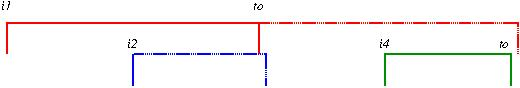
\includegraphics[width=.45\textwidth]{wiggling.jpg}
\end{center}
\caption{A timed behavior with two races}
\label{fig:races}
\end{figure}
\fi
This timed behavior contains two races, after two and four time units, respectively.
The first races is won by block $\{ 1, 3 \}$, and the second race is won by block $\{ 4, 5 \}$.
As a result of these races we cannot wiggle the timing of block $\{ 1, 3 \}$ by any amount:
if $i_1$ occurs just a bit later then timer $y$ must expire before timer $x$,
and if $i_1$ occurs just a bit earlier then timer $u$ must expire before timer $z$.
Note that when timer $x$ expires timer $y$ is stopped.
%
The above scenario is similar to the well-known Rush Hour puzzle game,
in which one has to slide blocking vehicles out of the way to find a path for one specific red car to exit a parking lot.
The next lemma asserts that we can always solve the puzzle for MMTs: for any timed behavior that contains races,
an equivalent timed behavior exists without races.
We may for instance slightly modify the timed behavior
\iflong
of Figure~\ref{fig:races} 
\fi
by scheduling block $\{ 2  \}$
a bit later and block $\{ 4, 5 \}$ a bit earlier.
Then all races have been eliminated and we can wiggle block $\{ 1, 3 \}$.

%We call a valuation $\tvals$ \emph{fraction-injective} if, for all distinct timers $x$ and $y$ in the domain of $\tvals$,
%the fractional parts of $x$ and $y$ are different.
%Note the any fraction-injective valuation is also injective.

\begin{lemma}
\label{race elimination}
Let $\sigma$ be any timed behavior.
Then there exists a timed behavior $\sigma'$ without races such that $\untime(\sigma)=\untime(\sigma')$.
\end{lemma}
\iflong
\begin{proof}
(Sketch) Let
\begin{eqnarray*}
\sigma & = & \tvals_0 \xrightarrow{d_1} \tvals'_0 \xrightarrow{i_1/o_1, \rho_1} \tvals_1 \xrightarrow{d_2} \tvals'_1 \xrightarrow{i_2/o_2, \rho_2} \tvals_2 \cdots
\xrightarrow{d_k} \tvals'_{k-1} \xrightarrow{i_k/o_k, \rho_k} \tvals_{k}.
\end{eqnarray*}
be a timed behavior.
%
For each index $j$, each timer in the domain of $\kappa_j$ has been started by some preceding event.
Let $\startedby_j : \domof{\kappa_j} \rightarrow \Pi_\sigma$ be the function that maps each timer in
the domain of $\kappa_j$ to the block that contains the event that started this timer.
Suppose that $\sigma$ contains a race, that is, there is an index $j>0$ and a timer $x$  
such that $\kappa'_{j-1}(x) = 0$ and $i_j \neq \toevent{x}$.
Let $B \in \Pi_\sigma$ be the block containing $j$. Then we say that block $B$ is the \emph{winner} of the race and block
$\startedby_{j-1}(x)$ is a \emph{loser}.
Note that whenever there is a race at $j$, this race has a single winner but it may have several losers.
Moreover, each block can be loser in at most one race.
A block that does not win any race can be wiggled forward by a small amount (if you don't win you might as well start later).
If block $B$ wins a race from block $B'$, then $\max(B)>\max(B')$, that is, $B$ contains an event that occurs later
in $\sigma$ than any event of $B'$.
This implies that the winning relation induces a partial order on the blocks of $\Pi_\sigma$.
Now consider the bottom elements in this partial order. These blocks do not win any race so we may wiggle them forward.
Once we have eliminated the bottom elements we can work our way upwards in the partial order and wiggle all blocks
forward one by one until no more races remain.
\end{proof}
\fi

%\marginpar{Races are sort of a limit case. I would like to state a corollary here that the set of timed behaviors that contain races have ``measure'' $0$. }

In a timed behavior, there is always an integer amount of time between events from the same block.
This means that, if we consider the absolute time at which events occur, the fractional part of the absolute times
of occurrence is the same for all events in a block.
We call a timed behavior \emph{transparent} if the fractional part of the absolute times of any pair of events from different blocks is different. Note that a transparent timed behavior contains no races.
\ifshort
We call a timed word $w$ \emph{transparent} if there exists a transparent timed behavior $\sigma$ with 
$w = \timedword(\sigma)$.
\fi

\begin{lemma}
\label{lemma: transparent timed behavior}
For each feasible untimed behavior $\beta$ there exists
a transparent timed behavior $\sigma$ such that $\beta = \untime(\sigma)$.
\end{lemma}
\iflong
\begin{proof}
Let $\beta$ be a feasible untimed behavior.
Then there exists a timed behavior $\sigma$ such that $\beta = \untime(\sigma)$.
By Lemma~\ref{race elimination}, we may assume that $\sigma$ contains no races.
By repeated application of Lemma~\ref{wiggle lemma}, we can wiggle the timing of all the blocks to make $\sigma$ transparent.
\end{proof}
\fi

\iflong
\paragraph{Causality maps.} 
Consider an untimed behavior
\begin{eqnarray*}
\beta & = & X_0 \xrightarrow{i_1/o_1, \rho_1} X_1  \xrightarrow{i_2/o_2, \rho_2} X_2 \cdots \xrightarrow{i_k/o_k, \rho_k} X_{k}.
\end{eqnarray*}
A causality map for $\beta$ is a function that specifies, for each timer that expires, the index of the event that
triggered this timeout.
Formally, let $T = \{ j \mid i_j \in \toevents \}$ be the set of indices of $\beta$ corresponding to a timeout.
A \emph{causality map} for $\beta$ is a function $c: T \rightarrow \{ 1 ,\ldots, k \}$ that assigns
to each index $j$ with $i_j = \toevent{x}$ an index $l < j$ such that $\rho_l$ starts $x$, and all events in between $i_l$ and $i_j$
do not affect $x$.

\begin{lemma}
\label{causality map untimed behavior}
Each untimed behavior $\beta$ that starts with the empty set of timers has a unique causality map $c$.
\end{lemma}
We say that $c$ is a causality map of a timed behavior $\sigma$ if it is a causality map of $\untime(\sigma)$,
and we say that it is a causality map of a timed run $\alpha$ if it is a causality map of $\beh(\alpha)$.
Lemma~\ref{causality map untimed behavior} implies that each timed run of an MMT has a unique causality map $c$.

\fi
Consider a timed word
$w  =   d_1 ~ i_1 ~ o_1 ~ d_2 ~ i_2 ~ o_2 \cdots d_k ~ i_k ~ o_k$.
We want to know, for each timeout event in $w$, by which event this timeout is triggered.
Let $T = \{ j \mid i_j = \mathit{to} \}$ be the set of indices corresponding to a timeout.
A \emph{causality map} for $w$ is a function $c: T \rightarrow \{ 1 ,\ldots, k \}$ that satisfies three conditions:
(1)
$c$ is injective (at most one timer is started on each transition),
(2)
for all $j$, $c(j) < j$ (a timeout is triggered by an earlier event), and
(3)
for all $j$, $\sum_{l=j+1}^{c(j)} d_l$ is an integer (timers expire after an integer delay).
\iflong
\begin{lemma}
\label{causality map run is causility map of its timed word}
Suppose $\alpha$ is a timed run of an MMT in which at most one timer is set
per transition and $c$ is the causality map of $\alpha$. 
Then $c$ is a causality map of $\timedword(\alpha)$.
\end{lemma}
\else
It is easy to see that a timed word has a causality map iff it is a timed word of an MMT that starts at most one timer
on each transition. 
\fi
In general, a timed word may have multiple causality maps.
\iflong
However, we have the following lemma.
Call a timed word \emph{transparent} if the fractional part of the absolute times of all input events in $I$ is different.

\begin{lemma}
\label{lemma unique causality map}
Suppose $\alpha$ is a timed run of an MMT in which at most one timer is set
per transition, $w =  \timedword(\alpha)$ and $w$ is transparent. 
Then $w$ has a unique causality map.
\end{lemma}
\else
However, a transparent timed word has a unique causality map.
\fi

Each timed word of MMT $\M$ with a unique causality map has a unique timed run that corresponds to it.
The causality map tells us which timers time out during the trace, so we have complete information
about the sequence of events that occurs. 
\iflong
A timed run of $\M$ is fully determined
by the sequence of time delays and events that occurs.

\begin{lemma}
\label{lemma unique timed run}
Suppose $w$ is a timed word of MMT $\M$ with a unique causality map.
Then there is a unique timed run $\alpha$ of $\M$ such that $w = \timedword(\alpha)$.
\end{lemma}

\fi
We are now prepared to prove our first main result:

\begin{theorem}
\label{timedimpliesuntimed}
Suppose that $\M$ and $\N$ are timer live MMTs in which at most one timer is started on each transition. Then
$\M \approx_{\mathit{timed}} \N$
implies
$\M \approx_{\mathit{untimed}} \N$.
\end{theorem}
\iflong
\begin{proof}
Suppose that $\M \approx_{\mathit{timed}} \N$.
Let $\beta$ be a feasible untimed behavior of $\M$.
For reasons of symmetry, it suffices to prove that $\N$ has a feasible untimed behavior $\beta'$ that is isomorphic to $\beta$.

Since $\beta$ be a feasible untimed behavior of $\M$, $\M$ has an untimed run $\gamma$ with $\beh(\gamma) = \beta$.
By Lemma~\ref{lemma: transparent timed behavior}, there exists a 
transparent timed behavior $\sigma$ such that $\beta = \untime(\sigma)$.
There exists a unique timed run $\alpha = \run(\gamma,\sigma)$ of $\M$ with $\untime(\alpha) = \gamma$ and $\beh(\alpha) = \sigma$.
Thus $\sigma$ is a timed behavior of $\M$.
Let  $w = \timedword(\alpha)$.
Then $w$ is a timed word of $\M$.
By Lemma~\ref{lemma unique causality map}, $w$ has a unique causality map $c$.
Since $\M \approx_{\mathit{timed}} \N$, $w$ is also a timed word of $\N$.
By Lemma~\ref{lemma unique timed run}, $\N$ has a unique time run $\alpha'$ such that $w = \timedword(\alpha')$.
Let $\beta' = \untime(\beh(\alpha'))$.
Then $\beta'$ is a feasible untimed behavior of $\N$.
Note that the mappings $\timedword$, $\untime$ and $\beh$ all preserve the number of events, the sequence of inputs that occur (except for the names of the timers in timeouts), and the sequence of outputs. Thus $\beta$ and $\beta'$ have the same length, the same inputs (except for the timer names), and the same outputs.
Moreover, by Lemmas~\ref{causality map untimed behavior} and \ref{causality map run is causility map of its timed word},
$\beta'$ and $\beta$ have the same causality map $c$.

By induction on the number of events in $\beta$ and $\beta'$, we prove that they are isomorphic.
Since $\approx_{\mathit{untimed}}$ is symmetric, this suffices to prove the theorem.

Induction base. If $\beta$ and $\beta'$ contain $0$ events then they are both equal to the empty set of variables $\emptyset$,
and thus trivially isomorphic.

For the induction step, suppose $\beta$ and $\beta'$ contain $k+1$ events:
\begin{eqnarray*}
\beta & = & X_0 \xrightarrow{i_1/o_1, \rho_1} X_1  \xrightarrow{i_2/o_2, \rho_2} X_2 \cdots \xrightarrow{i_k/o_k, \rho_k} X_{k}
 \xrightarrow{i_{k+1}/o_{k+1}, \rho_{k+1}} X_{k+1},\\
\beta' & = & Y_0 \xrightarrow{i'_1/o_1, \tau_1} Y_1  \xrightarrow{i'_2/o_2, \tau_2} Y_2 \cdots \xrightarrow{i'_k/o_k, \tau_k} Y_{k} 
 \xrightarrow{i'_{k+1}/o_{k+1}, \tau_{k+1}} Y_{k+1}.
\end{eqnarray*}
Let $\delta$ and $\delta'$ be the prefixes of $\beta$ and $\beta'$, respectively,
containing $k$ events. Then $\delta$ is also a feasible untimed behavior and, by
induction hypothesis, there exists an isomorphism $f = f_0 ,\ldots, f_k$ such that $\delta' = f(\delta)$.
Our task is to extend this isomorphism to $\beta$ and $\beta'$.

Since $\timedword$, $\untime$ and $\beh$ preserve inputs except for the timers in timeouts,
either $i_{k+1} = i'_{k+1} \in I$ or $i_{k+1}, i'_{k+1} \in\toevents$.
If $i_{k+1} = \toevent{x}$, for some $x \in X_k$, then $i_{k+1}$ is triggered by a previous event $i_j$ with $j=c(k+1)$ that started
timer $x$, and this timer was left unaffected by all events from $\beta$ in between $i_j$ and $i_{k+1}$. In this case,
$i'_{k+1} = \toevent{x'}$, for some $x' \in X_k$, and $i'_{k+1}$ is triggered by a previous event $i'_j$ with $j=c(k+1)$ that started
timer $x'$, and this timer was left unaffected by all events from $\beta'$ in between $i_j$ and $i_{k+1}$.
Using the definition of an isomorphism, we may infer that $i'_{k+1} = \toevent{f_k(x)}$.

Now suppose that $x \in X_{k+1}$ is a timer that is active after $\beta$.
Then, since $\M$ is timer live, there exists an untimed behavior $\beta_x$ consisting of transitions that leave $x$ unaffected, except for the last one in which $x$ expires, and such that $\beta \cdot \beta_x$ is a feasible untimed behavior of $\M$.
Using the same construction as in the beginning of this proof, we may construct an untimed behavior $\beta'_x$ such
that $\beta' \cdot \beta'_x$ is a feasible untimed behavior of $\N$ such that $\beta \cdot \beta_x$ and $\beta' \cdot \beta'_x$
have the same length, the same inputs (except for the timer names) and the same causality map $c_x$.
Let $m$ be the index of the final event in $\beta' \cdot \beta'_x$. Then $m$ is in the domain of $c_x$ and $c_x(m) \leq k+1$.
If $c_x(m) \leq k$ then we define $f_{k+1}(x) = f_k (x)$.
Otherwise, if $c_x(m) = k+1$ then we know that timer $x$ is started in the last transition of $\beta$.
Since $c_m$ is also a causality map for $\beta'$, there is also a unique timer $x' \in Y_{k+1}$ that is started in the last transition of $\beta'$.
In this case, we define $f_{k+1}(x) = x'$.
Repeating this construction for all timers $x \in X_{k+1}$, we define a function $f_{k+1} : X_{k+1} \rightarrow Y_{k+1}$ and thus
extend isomorphism $f$ to $\beta$ and $\beta'$.
Note that $f_{k+1}$ is surjective because for each $y \in Y_{k+1}$, since $\N$ is timer live,
there exists an untimed behavior $\beta_y$ consisting of transitions that leave $y$ unaffected, except for the last one in which $y$ expires, and such that $\beta' \cdot \beta_y$ is a feasible untimed behavior of $\N$.
Using again the same construction as in the beginning of this proof, we may establish that $X_{k+1}$ contains a corresponding timer. 
\end{proof}
\fi

In the remainder of this article, we only consider timer live MMTs in which at most one timer is started on each transition,
which means we may assume equivalence of the timed and the untimed semantics.
